\section{Recognizable implies regular}\label{sec:rec->reg}


\begin{theorem}\label{thm:Rec->Reg}
If a language of $\TWT$-graphs is recognizable, then it is regular.
\end{theorem}

 

\subsection{Preliminaries}

We define below guarded modules. Intuitively, a module is guarded if it is pure of some type $\tau$ and whenever we replace it with a letter, this  letter is $\tau$-guarded in the obtained graph.
\begin{definition}[Strict modules, Guarded modules]
Let $G$ be a graph and $M$ a module of $G$.
 We say that $M$ is \emph{strict} if it does not contain all the edges and vertices of $G$.
 We say that $M$ is \emph{guarded} if it is pure and:
\begin{itemize}
\item   $M$ is maximal, if $M$ is parallel or test,
\item $M$ is parallel to another module of $G$, if $M$ is series.
\end{itemize}
\end{definition}

The following lemma follows from the definition of guarded modules. 

\begin{lemma}\label{lem:meaning-of-guared-module}
Let $G$ be a graph, $M$ a guarded module of $G$ of type $\tau$, and  $x$ a letter of the same arity as $M$. We denote by $G[x/M]$ the graph obtained by replacing the module $M$ by an $x$-labeled edge whose interface is that of $M$.  
The letter $x$ is $\tau$-guarded in $G[x/M]$.
\end{lemma}





We will not show Thm.~\ref{thm:Rec->Reg} directly, but we will proceed gradually, by showing that this result holds for three sub-classes of $\TWT$ graphs. First for \emph{alternating-free domain-free graphs}, for \emph{domain-free} graphs (which we define below), then for domain graphs. We finally lift these results to the whole class of $\TWT$ graphs. 

\begin{definition}[Domain-free, alternation-free graphs]
A graph is \emph{domain-free} if all its domain modules are atomic. A graph is \emph{alternation-free} if it has no strict guarded module.  
\end{definition}

 In all these steps, we use the following lemma:
\begin{lemma}\label{lem:imposing-type-is-recognizable}
Let $L$ be a language of $\TWT$-graphs, $x$ a letter and $\tau$ a type. If $L$ is recognizable then the restriction of $L$ to the graphs of type $\tau$ (resp.  the graphs where $x$ is $\tau$-guarded, word graphs, multiset graphs, domain-free graphs, alternation-free graphs) is also recognizable.
\end{lemma}

\begin{lemma}\label{lem:structure-of-guarded-modules} In a domain-free graph, every two guarded modules are either independent or module one of the other.

In an arbitrary graph, every two domain modules are either independent or module one of the other.
\end{lemma}
\begin{lemma}\label{lem:tau-modules-substitution-domain-free} Let $G, H$ be domain-free graphs, $x$ a letter  and suppose that $H$ is pure and $G[H/x]$ is a guarded substitution. We have the following equality:
$$\mathsf{guarded\text{-}modules}(G[H/x])\ =\ \mathsf{guarded\text{-}modules}(G)[H/x]\ \cup\ \mathsf{guarded\text{-}modules}(H)\cup \set{H}$$
\end{lemma}
\begin{lemma}\label{lem:tau-modules-substitution-domain} Let $G, H$ be domain graphs, $x$ a unary letter. We have the following equality:
$$\mathsf{domain\text{-}modules}(G[H/x])\ =\ \mathsf{domain\text{-}modules}(G)[H/x]\ \cup\ \mathsf{domain\text{-}modules}(H)$$
\end{lemma}
\todo{define domain-modules and guarded-modules}
\todo{algebras are ranked now}
\todo{domain free are basically series-parallel}
%\begin{proof}
%
%\end{proof}

%\begin{lemma}
%Let $\A$ be a $\sigma$-algebra recognizing a language $L$. There is a $\sigma$-algebra $\B$ whose domain can be partitioned into $D_1$ and $D_2$, and a homomorphism $h$ 
% \end{lemma}

\subsection{Alternation-free domain-free graphs}

\begin{lemma}\label{lem:alt-free-dom-free-description}
If $G$ is an alternation-free domain-free $\TWT$ graph, then $G=H[\vec{T}/\vec{x}]$ where 
\begin{itemize}
\item $H$ is either a word or a multiset graph,
\item $\vec{T}$ are multiset graphs of type test not containing the letters $\vec{x}$ and 
\item  the  letters of $\vec{x}$ are $\mathsf{t}$-guarded in $G$.
\end{itemize}  
\end{lemma}
%\begin{proof}
%\todo{complete}
%\end{proof}

\begin{proposition}\label{prop:rec->reg-alt-free-dom-free}
If a language of alternation-free domain-free $\TWT$ graphs is recognizable, then it is regular.
\end{proposition}
\begin{proof}
Let $L$ be a language of non-alternating domain-free graphs, $\A$ an algebra of domain $D$, $h:\mathbb{G}_\TWT(\Sigma) \to \A$ a homomorphism and $F\subseteq D$ such that $h^{-1}(F)=L$. We denote by $L_v$ the set of graphs whose image by $h$ is $v$. Note that we have the following equality:
 $$L\ =\ \underset{f\in F}{\cup} L_f.$$ 
We show in the following that $L_v$ is regular for every $v\in D$, and this is enough to conclude. 
\medskip

For every $v\in D$, we associate a new letter $x_v$, and denote this new set of letters by $\Gamma$.  We extend the homomorphism $h$ to $\TWT$-graphs over the alphabet $\Sigma \cup \Gamma$ by letting $h(x_v)=v$ for every $x_v\in\Gamma$. 

For every $v\in D$, let $T_{v}$ be the set of multiset graphs over $\Sigma$ of type test  whose image by $h$ is $v$, and let $M_{v}$ be the set of word or multiset graphs over  $\Sigma\cup \Gamma$, where the letters of $\Gamma$ are $\mathsf{t}$-guarded.  Using Lem.~\ref{lem:alt-free-dom-free-description}, we have:
$$ L_v=M_v[T_w/x_w,\  w\in D]$$ 
By Lem.~\ref{lem:imposing-type-is-recognizable} and using the fact that recognizability implies regularity for word and multiset graphs, we conclude that $L_v$ is regular for every $v\in D$.
\end{proof}

\subsection{Domain-free graphs}
 



\begin{proposition}\label{prop:rec->reg-dom-free}
If a language of domain-free graphs is recognizable, then it is regular.
\end{proposition}
\begin{proof}
Let $L$ be a language of domain-free graphs, $\A$ an algebra of domain $D$, $h:\mathbb{G}_\TWT(\Sigma) \to \A$ a homomorphism and $F\subseteq D$ such that $h^{-1}(F)=L$. Let us show that $L_v$, the set of graphs over $\Sigma$ whose image (by $h$) is $v$,  is regular for every $v\in D$. 
\medskip

We associate every $v\in D$ with two new letters $x_v$ and $y_v$ of the same arity as $v$, and let  $\Gamma:=\set{x_v\ | \ v\in D}$ and $\Delta:=\set{y_v\ | \ v\in D}$. If $Q\subseteq D$, we denote by $X_D$ and $Y_D$ the subsets of $\Gamma$ and $\Delta$ corresponding to these elements.   We extend the homomorphism $h$ to $\TWT$ graphs over the alphabet $\Sigma \cup \Gamma \cup \Delta$ by letting $h(x_v)=h(y_v)=v$ for every $x_v\in\Gamma$ and $y_v\in\Delta$.
\medskip

Let $v\in D$, $Q, R\subseteq D$, $X\subseteq \Gamma$, and $Y\subseteq \Delta$.  We define the set of graphs $L^{Q,R,X,Y}_{v}$ as follows. A graph  $G$ is in this set if and only if:

\begin{itemize}
\item $G$ is a domain-free graph over the alphabet $\Sigma\cup X\cup Y$, 
\item the image of $G$ is $v$,
\item  the image of the strict guarded series modules of $G$ belong to $Q$, 
\item   the image of the strict guarded parallel modules of $G$ belong to $R$, 
\item the letters of $X$ are $\mathsf{s}$-guarded  in $G$ ,
\item the letters of $Y$ are $\mathsf{p}$-guarded in $G$.  
\end{itemize}
\smallskip

 Let $S^{Q,R,X,Y}_{v}$ and $P^{Q,R,X,Y}_{v}$ be the restriction of $L^{Q,R,X,Y}_{v}$ to series and parallel graphs respectively. Let us show that these two languages are regular  when $X\cap X_Q=\emptyset$ and $Y\cap Y_Q=\emptyset$. We proceed by induction on the size of $Q\cup R$. When $Q=R=\emptyset$, the graphs of these sets are   alternation-free. Using Lemma~\ref{lem:imposing-type-is-recognizable} and Prop~\ref{prop:rec->reg-alt-free-dom-free}, we conclude the base case. 
 \medskip
 
  To handle the inductive case, we show the following equalities:
\begin{align*}
S^{Q\cup\set{w},R,X,Y}_v=&S^{Q,R,X\cup\set{x_w},Y}_v[\mu x_w. S^{Q,R,X\cup\set{x_w},Y}_w/x_w][S^{Q,R,X,Y}_w/x_w]\qquad (\dagger)\\[5pt]
S^{Q,R\cup\set{w},X,Y}_v=&S^{Q,R,X,Y\cup\set{y_w}}_v[\mu y_w. P^{Q,R,X,Y\cup\set{y_w}}_w/y_w][P^{Q,R,X,Y}_w/y_w]\\[5pt]
P^{Q\cup\set{w},R,X,Y}_v=&P^{Q,R,X\cup\set{x_w},Y}_v[\mu x_w. S^{Q,R,X\cup\set{x_w},Y}_w/x_w][S^{Q,R,X,Y}_w/x_w]\\[5pt]
P^{Q,R\cup\set{w},X,Y}_v=&P^{Q,R,X,Y\cup\set{y_w}}_v[\mu y_w. P^{Q,R,X,Y\cup\set{y_w}}_w/y_w][P^{Q,R,X,Y}_w/y_w]
\end{align*}
Let us show the  equality $(\dagger)$, the others are similar. The right-to-left implication follows from these inclusions which are consequence of Lem.~\ref{lem:tau-modules-substitution}:

\begin{itemize}
\item $\mu x_w. S^{Q,R,X\cup\set{x_w},Y}_w\subseteq S^{Q\cup\set{w},R,X\cup\set{x_w},Y}_w$,\\[-5pt]
\item $S^{Q,R,X\cup\set{x_w},Y}_v[S^{Q\cup\set{w},R,X\cup\set{x_w},Y}_w/x_w]\subseteq S^{Q\cup\set{w},R,X\cup\set{x_w},Y}_v$,\\[-5pt]
\item $S^{Q\cup\set{w},R,X\cup\set{x_w},Y}_v[S^{Q,R,X,Y}_w/x_w]\subseteq S^{Q\cup\set{w},R,X,Y}_v$.
\end{itemize}

Let us show the other direction. We call $w$-module of a graph $K$ a series module of $K$ whose image by $h$ is $w$. The $w$-normal-form of a graph $K$ is the graph obtained from $K$ by recursively replacing its strict $w$-modules by the letter $x_w$. This operation yields always the same graph thanks to Lem.~\ref{lem:structure-of-guarded-modules}.   
 Let $H$ be the $w$-normal-form of $G$, $M$ be the set of $w$-normal-forms of its strict $w$-modules and $N$ the set of $w$-modules of $G$ with no strict $w$-modules.
 
 
 The picture below illustrates these constructions. In the graph $G$, the colored modules are the $w$-modules of $G$. 
 \begin{center}
 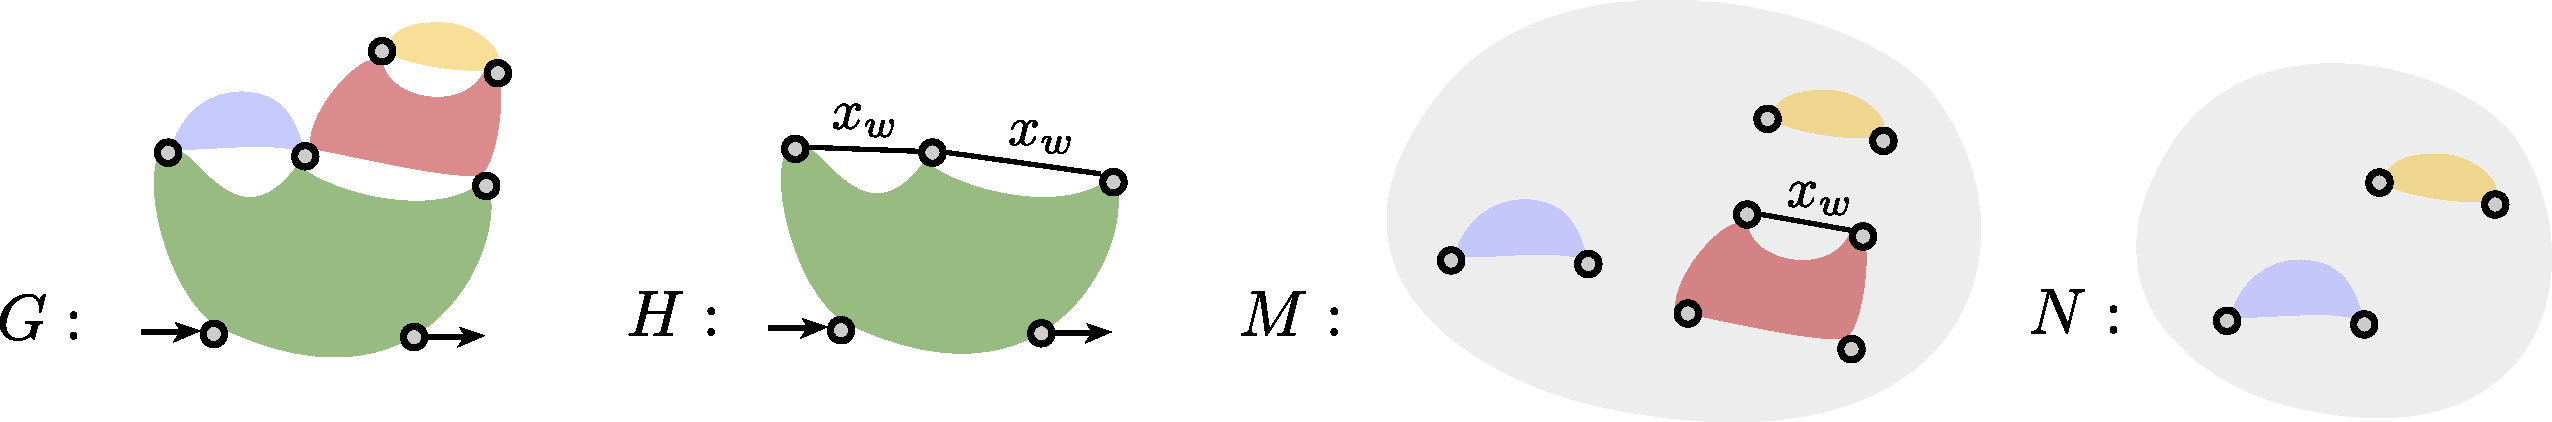
\includegraphics[scale=.3]{Pictures/proof-rec->reg-dom-free}
\end{center}
We have that $G\subseteq H[\mu x_w. M/x_w][N/x_w]$. Note that 
$M\subseteq $  and $N\subseteq$ . In particular the letter $x_w$ is $\mathsf{s}$-guarded in $M$ thanks to Lem.~\ref{lem:meaning-of-guared-module}. This concludes the left-to-right implication of $(\dagger)$.
\medskip

\noindent Finally, notice that for every $v\in D$, we have:
$$ L_v=L^{\emptyset,\emptyset,\Gamma,\Delta}_v[S^{D,D,\emptyset,\emptyset}_w/x_w, w\in D] [S^{D,D,\emptyset,\emptyset}_w/y_w, w\in D]$$
The set $L^{\emptyset,\emptyset,\Gamma,\Delta}_v$ is a set of alternation-free and domain-free graphs, its regularity follows from Lem.~\ref{lem:imposing-type-is-recognizable} and Prop.~\ref{prop:rec->reg-alt-free-dom-free}.
\end{proof}

\subsection{Domain graphs}

\begin{lemma}\label{lem:domain-modules-atomic->domain-free}
Let $G$ be a domain graph whose strict domain modules, are all atomic. There is a domain-free graph $H$ such that $G=\dom(H)$.   
\end{lemma}



\begin{proposition}\label{prop:rec->reg-dom}
If a language of domain graphs is recognizable, then it is regular.
\end{proposition}
\begin{proof}
Let $L$ be a language of domain graphs, $\A$ an algebra whose domain is $D$, $h:\mathbb{G}_\TWT(\Sigma) \to \A$ a homomorphism and $F\subseteq D$ such that $h^{-1}(F)=L$. Let us show that $L_v$, the set of graphs over $\Sigma$ whose image  is $v$,  is regular for every $v\in D$. 
\medskip

We associate every $v\in D$ with a new letter $x_v$ whose arity is the same as $v$ and we let  $\Gamma:=\set{x_v\ | \ v\in D}$. If $Q\subseteq D$, we denote by $X_D$ the letters of $\Gamma$ corresponding to these elements.   We extend the homomorphism $h$ to $\TWT$-graphs over the alphabet $\Sigma \cup \Gamma$ by letting $h(x_v)=v$ for every $x_v\in\Gamma$. 
\medskip

Let $v\in D$, $Q\subseteq D$ and $X\subseteq \Gamma$.  We define the set of graphs $L^{Q,X}_{v}$, by letting a graph $G$ in this set  if and only if:
\begin{itemize}
\item $G$ is a domain graph over the alphabet $\Sigma\cup X$, 
\item the image of $G$ is $v$,
\item  the image of the strict domain modules of $G$ belong to $Q$.
\end{itemize}


 Let us show that $L^{Q,X}_v$ is regular. This is enough to conclude since $L_v=L^{D,\emptyset}_v$.
\medskip

 We proceed by induction on the size of $Q$. Let $X\subseteq \Gamma$ and suppose that $Q=\emptyset$. For every $w\in D$, let $M_w$ be the set of domain-free graphs over the alphabet $\Sigma\cup X$ whose image is $w$.  The set $M_w$ is the restriction of $h^{-1}(w)$ to those graphs which are domain-free. By Lem.~\ref{lem:imposing-type-is-recognizable}, $M_w$ is recognizable. Using Prop.~\ref{prop:rec->reg-dom-free}, $M_v$ is regular. 
 \medskip
 
 By Lem.~\ref{lem:domain-modules-atomic->domain-free}, we have the following equation:
$$ L^{\emptyset, X}_v= \bigcup_{\substack{w\in D\\ \dom(w)=v}}\dom(M_w)$$
The set  $ L^{\emptyset, X}_v$ is regular because $M_w$ is regular, which concludes the base case.  
\medskip
 
 To handle the inductive case, we show the following equality:
 $$L^{Q\cup\set{w}, X}_v= L^{Q, X\cup\set{x_w}}_v[\mu x_w.\ L^{Q, X\cup\set{x_w}}_w/x_w][L^{Q, X}_w/x_w] \qquad (\dagger)$$
 The right-to-left implication holds because of the following inclusions, which follow from Lem.~\ref{lem:tau-modules-substitution}:\\[-.5pt]
 \begin{itemize}
 \item $\mu x_w.\ L^{Q, X\cup\set{x_w}}_w\subseteq L^{Q\cup\set{w}, X\cup\set{x_w}}_w$,\\[-.5pt]
 \item $L^{Q, X\cup\set{x_w}}_v[L^{Q\cup\set{w}, X\cup\set{x_w}}_w/x_w]\subseteq L^{Q\cup\set{w}, X\cup\set{x_w}}_v$,\\[-.5pt]
 \item  $L^{Q\cup\set{w}, X\cup\set{x_w}}_v[L^{Q, X}_w/x_w]\subseteq L^{Q\cup\set{w}, X}_v$.
 \end{itemize}
 
 Let us prove the other direction. Let $G\in L^{Q\cup\set{w}, X}_v$
 We define the graph $H$ and the sets of graphs $S$ and $T$ as follows. 
 
 We call $w$-module of a graph $K$ a domain module of $K$ whose image by $h$ is $w$. The $w$-normal-form of a graph $K$ is the graph obtained from $K$ by recursively replacing its strict $w$-modules by the letter $x_w$.  
 Let $H$ be the $w$-normal-form of $G$, $S$ the set of $w$-normal-forms of its strict $w$-modules and $T$ the set of $w$-modules of $G$ with no strict $w$-modules.
 
 
 The picture below illustrates these constructions. In the graph $G$, the inner vertices which are drawn are the interfaces of all domain modules whose image by $h$ is $w$. 
 \begin{center}
 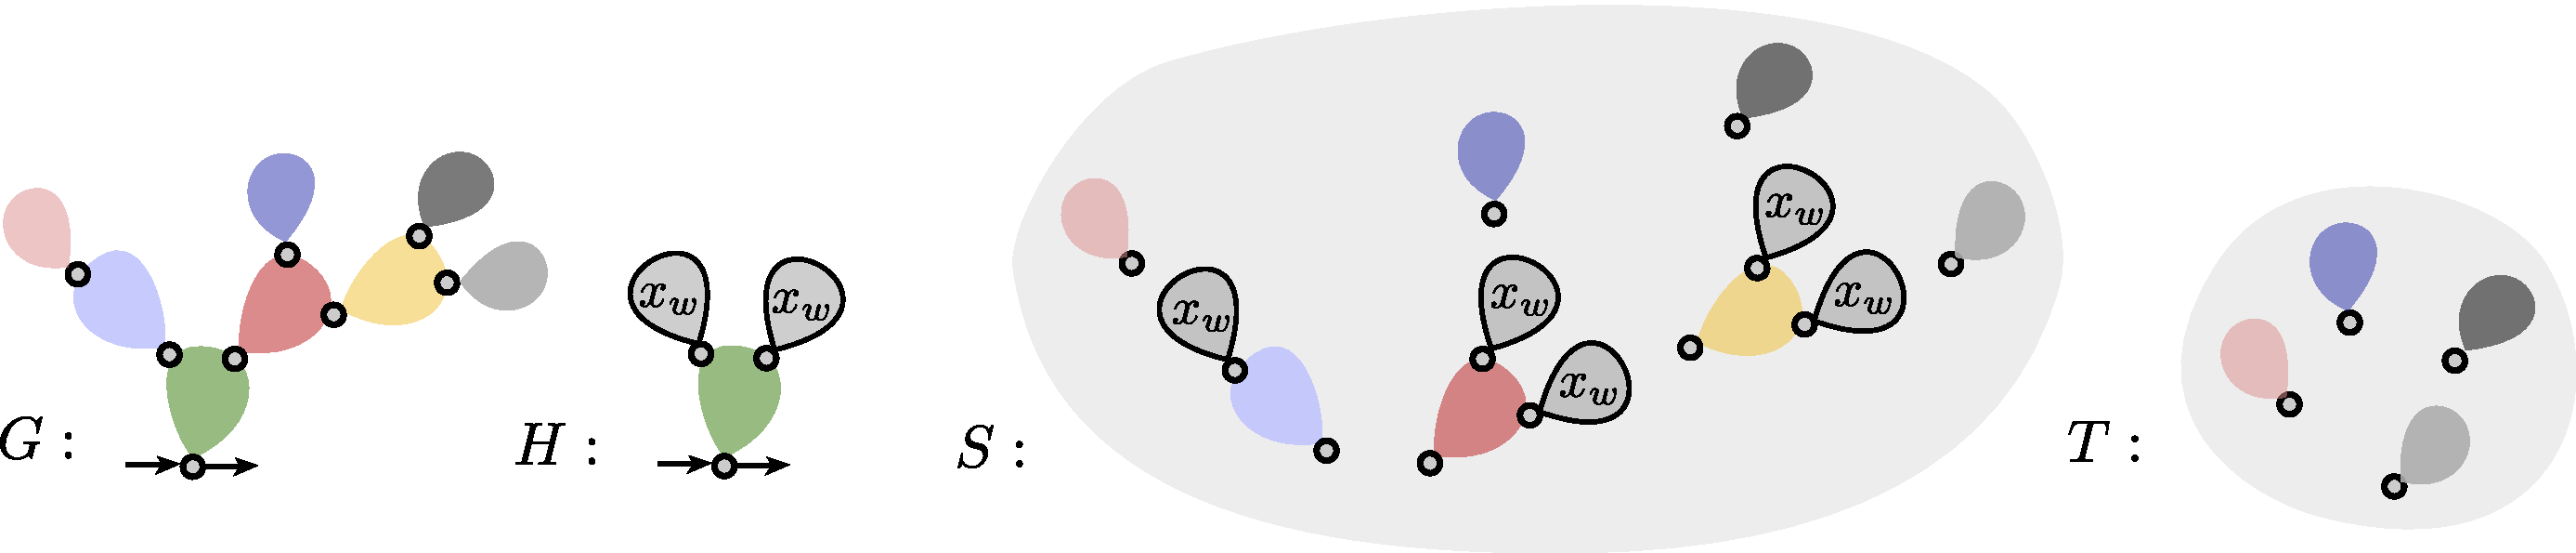
\includegraphics[scale=.3]{Pictures/proof-rec->reg-dom}
\end{center}
We have that $G\subseteq H[\mu x_w. S/x_w][T/x_w]$, which concludes the left-to-right implication.
\medskip

The iteration and substitutions in $(\dagger)$ are guarded because the languages which we iterate and substitute and domain languages, and the variable $x_w$ is unary. Since the languages $L^{Q, X\cup\set{x_w}}_v$, $L^{Q, X\cup\set{x_w}}$ and $L^{Q, X}_w$ are regular by induction hypothesis, we conclude that $L^{Q\cup\set{w}, X}_v$ is also regular. 
\end{proof}

\subsection{$\mathsf{TW}_2$ graphs}

\begin{lemma}\label{structure-of-twt-graphs}
If $G$ is a $\TWT$-graph, then $G=H[\vec{D}/\vec{x}]$ where $H$ is domain-free and $\vec{D}$ are domain graphs. 
\end{lemma}

Now we are ready to prove Thm.~\ref{thm:Rec->Reg}.
\begin{proof}[Proof of Thm.~\ref{thm:Rec->Reg}]
Let $L$ be a language of $\TWT$-graphs, $\A$ an algebra whose domain is $D$, $h:\mathbb{G}_\TWT(\Sigma) \to \A$ a homomorphism and $F\subseteq D$ such that $h^{-1}(F)=L$. Let us show that $L_v$, the set of graphs over $\Sigma$ whose image  is $v$,  is regular for every $v\in D$. 
\medskip

We associate every $v\in D$ with a new letter $x_v$ whose arity is the same as $v$ and we let  $\Gamma:=\set{x_v\ | \ v\in D}$.   We extend  $h$ to $\TWT$-graphs over the alphabet $\Sigma \cup \Gamma$ by letting $h(x_v)=v$ for every $x_v\in\Gamma$. 
\medskip

For every $v\in D$, we let $M_v$ be the set of domain-free graphs over the alphabet $\Sigma\cup \Gamma$ whose image is $v$, and let $N_v$ be the set of domain graphs over the alphabet $\Sigma$ whose image is $v$. The set $M_v$ is the restriction of $h^{-1}(v)$ to those graphs which are domain-free, hence it is recognizable by Lem.~\ref{lem:imposing-type-is-recognizable}. Similarly, $N_v$ is also recognizable. Hence, by Prop.~\ref{prop:rec->reg-dom-free} and Prop.~\ref{prop:rec->reg-dom} they are both regular.  

\medskip
We have the following equation, consequence of Lem.~\ref{structure-of-twt-graphs}:
$$ L_v=M_v[N_w/x_w, w\in D]$$
Substitutions in the equation above are guarded because $N_w$ is of type domain and $x_w$ is unary.  Since $M_v$ and $N_w$ are regular, the language $L_v$ is also regular.
\end{proof}
\begin{remark}
By analyzing this proof, we see that we never use iteration over test graphs. 
\end{remark}